\documentclass[aspectratio=169]{beamer}

% Modern, Minimalist Theme
\usetheme[progressbar=frametitle,block=fill]{metropolis}

% Packages
\usepackage{graphicx}
\usepackage{booktabs}
\usepackage{amsmath}
\usepackage{xcolor}
\usepackage{colortbl}
\usepackage{fontawesome5}

% Custom Dark Mode Color Palette
\definecolor{DarkBg}{HTML}{0d1117}        % Deep Charcoal/Slate
\definecolor{ElectricMint}{HTML}{00df94}  % Primary Accent
\definecolor{SoftGold}{HTML}{eb811b}      % Secondary Accent / Alerts
\definecolor{SilverText}{HTML}{e6edf3}    % Main Text
\definecolor{HighlightDark}{HTML}{1a2332} % Subtle Table Highlight

% Apply Colors to Beamer Elements
\setbeamercolor{background canvas}{bg=DarkBg}
\setbeamercolor{normal text}{fg=SilverText}
\setbeamercolor{frametitle}{bg=DarkBg, fg=ElectricMint}
\setbeamercolor{progress bar}{fg=ElectricMint, bg=SilverText!30}
\setbeamercolor{title separator}{fg=ElectricMint}
\setbeamercolor{alerted text}{fg=SoftGold}
\setbeamercolor{itemize item}{fg=ElectricMint}
\setbeamercolor{itemize subitem}{fg=ElectricMint}

% Block Colors (Flat Design)
\setbeamercolor{block title}{bg=HighlightDark, fg=ElectricMint}
\setbeamercolor{block body}{bg=DarkBg, fg=SilverText}

% Title details
\title{\Huge Traffic Signal Optimization}
\subtitle{\vspace{0.2cm}\large \textcolor{ElectricMint}{using Reinforcement Learning} \\ \vspace{0.4cm} \small M.Tech / Thesis Presentation}
\author{
  Rohit Kumar (CS23B2053) \and 
  Gyan Chandra (CS23I1053) \and 
  Sarvan Kumar (ME23B1065)
}
\institute{
  \vspace{0.3cm}
  \textbf{Instructor:} Dr. Rahul Raman \\
  \vspace{0.2cm}
  Indian Institute of Information Technology, Design and Manufacturing, Kancheepuram
}
\date{\today}

\begin{document}

% 1. Title Slide
\begin{frame}[plain]
  \titlepage
\end{frame}

% 2. Introduction
\begin{frame}{The Problem \& The Solution}
  \begin{block}{The Bottleneck \faTrafficLight}
    Traditional fixed-time controllers use static phase sequences. They operate blindly and fail to adapt to real-time, dynamic traffic demand, causing severe congestion and economic loss.
  \end{block}
  \vspace{0.3cm}
  \begin{block}{The Data-Driven Solution \faBrain}
    Reinforcement Learning (RL) allows an agent to continuously interact with the environment. It automatically learns optimal signal control policies purely by observing queues and penalizing delays.
  \end{block}
\end{frame}

% 3. Environment Design
\begin{frame}{Environment Architecture}
  \begin{columns}
    \column{0.55\textwidth}
    \textbf{Simulation Framework}
    \begin{itemize}
      \item \textbf{Engine:} Eclipse SUMO (Simulation of Urban MObility)
      \item \textbf{Topology:} 4-way Indian urban intersection
      \item \textbf{Ruleset:} Left-Hand Drive (LHD), Two lanes per arm
      \item \textbf{Control Interface:} Phase-based signal plan taking discrete actions at fixed decision intervals.
    \end{itemize}
    
    \column{0.45\textwidth}
    \begin{figure}
        \centering
        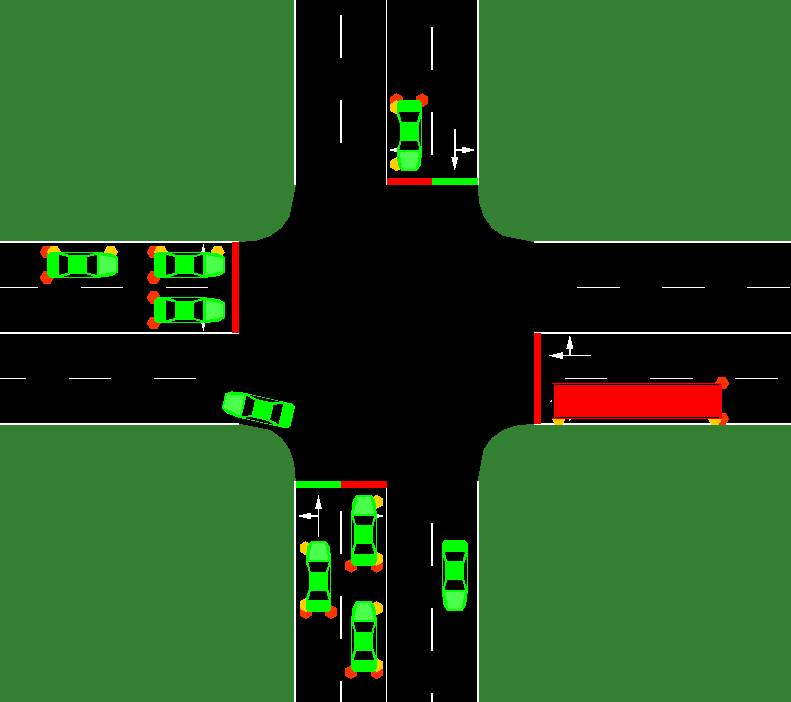
\includegraphics[width=0.9\textwidth]{intersection_map.png}
    \end{figure}
  \end{columns}
\end{frame}

% 4. MDP Formulation
\begin{frame}{Mathematical MDP Formulation}
  The traffic control problem is an MDP: $\mathcal{M}=\langle \mathcal{S},\mathcal{A},\mathcal{P},\mathcal{R},\gamma \rangle$.

  \vspace{0.5cm}
  \textbf{State Space (6D Macroscopic Vector):}
  \[ S_t = [Q_{NS}, Q_{EW}, W_{NS}, W_{EW}, P, T_{elapsed}] \]
  \begin{itemize}
      \item \textcolor{ElectricMint}{$Q$}: Directional queue lengths.
      \item \textcolor{ElectricMint}{$W$}: Directional waiting-time aggregates.
      \item \textcolor{ElectricMint}{$P$}: Active phase index \quad|\quad \textcolor{ElectricMint}{$T_{elapsed}$}: Elapsed time in phase.
  \end{itemize}

  \vspace{0.5cm}
  \textbf{Action Space (5 Discrete Actions):}
  \[ A = \{0, 1, 2, 3, 4\} \]
  {\small Action 0 holds the current phase. Actions 1-4 transition to specific phases.}
\end{frame}

% 5. Reward Optimization (Ablation Study)
\begin{frame}{Reward Function Ablation Study}
  \textbf{Objective:} Find the mathematical equilibrium between congestion and flow.
  \[ R_t = -w_1\,\Delta W_t - w_2\,Q_t - w_3\,C_t + w_4\,T_t \]
  
  \vspace{0.2cm}
  \begin{table}
  \centering
  \renewcommand{\arraystretch}{1.2}
  \resizebox{0.9\textwidth}{!}{
  \begin{tabular}{lccc}
  \toprule
  \textbf{Scenario} & \textbf{Reward Signal} & \textbf{Queue \faCar} & \textbf{Throughput \faRocket} \\
  \midrule
  Baseline & -1608.30 & 11.97 & 183.00 \\
  Queue Focused & -3513.00 & 11.40 & 194.00 \\
  \rowcolor{HighlightDark} \textbf{\textcolor{ElectricMint}{Wait Focused (Winner)}} & \textbf{\textcolor{ElectricMint}{-1144.80}} & \textbf{\textcolor{ElectricMint}{11.80}} & \textbf{\textcolor{ElectricMint}{217.00}} \\
  Balanced Aggressive & -2280.00 & 11.59 & 208.00 \\
  \bottomrule
  \end{tabular}
  }
  \end{table}

  \vspace{0.2cm}
  \small \textbf{Optimal Weights Adopted:} Wait=0.8, Queue=0.2, Switch=2.0, Throughput=1.0.
\end{frame}

% 6. Algorithms
\begin{frame}{Algorithmic Landscape}
  \begin{columns}[T]
    \column{0.5\textwidth}
    \textbf{Value-Based Methods}
    \begin{itemize}
      \item \textbf{Q-Learning:} Tabular TD-learning. Prone to overestimation.
      \item \textbf{Double Q-Learning:} Decouples selection and evaluation. Eliminates bias.
      \item \textbf{DQN:} Neural Q-table approximation via Replay Buffers and Target Networks.
    \end{itemize}
    
    \column{0.5\textwidth}
    \textbf{Policy Gradient Methods}
    \begin{itemize}
      \item \textbf{A2C:} Uses Advantage $A(s,a)$ to dramatically reduce variance.
      \item \textbf{PPO:} Implements a Clipped Surrogate Objective for safe updates.
      \item \textbf{TRPO:} Enforces a strict KL-Divergence Trust Region ($\mathbb{E}[ D_{KL} ] \le \delta$) for monotonic stability.
    \end{itemize}
  \end{columns}
\end{frame}

% 7. Training Infrastructure
\begin{frame}{Large-Scale Training Infrastructure}
  \begin{itemize}
    \item \textbf{Scale:} All 7 algorithms underwent identical, rigorous training pipelines for \textbf{300 episodes} to guarantee absolute convergence.
    \vspace{0.4cm}
    \item \textbf{State Normalization (Welford's Algorithm):}
    \begin{itemize}
        \item Raw waiting times heavily skew neural networks (values $>$ 1000).
        \item Online running mean/variance scaling dynamically standardizes inputs.
        \item \textcolor{SoftGold}{Critical mechanism} to prevent catastrophic gradient explosions in PPO and TRPO architectures.
    \end{itemize}
    \vspace{0.4cm}
    \item \textbf{Topological Efficiency:} 
    \begin{itemize}
        \item Our compact 6D macroscopic state space allowed highly efficient, CPU-friendly networks ($64 \times 64$ hidden layers).
    \end{itemize}
  \end{itemize}
\end{frame}

% 8. Results Table
\begin{frame}{Final Performance Metrics (300 Episodes)}
  \begin{table}
  \centering
  \renewcommand{\arraystretch}{1.2}
  \resizebox{1.0\textwidth}{!}{
  \begin{tabular}{lccccc}
  \toprule
  \textbf{Agent} & \textbf{Queue \faCar} & \textbf{Wait \faClock} & \textbf{Throughput \faRocket} & \textbf{Delay \faHourglassHalf} & \textbf{Reward} \\
  \midrule
  Fixed-Time & 14.22 & 6.79s & 188.0 & 8.92s & -1821.70 \\
  Q-Learning & 11.71 & 4.47s & 191.0 & 6.72s & -1636.60 \\
  \rowcolor{HighlightDark} \textbf{Double Q} & \textbf{11.11} & 4.57s & \textbf{\textcolor{ElectricMint}{200.0}} & 6.81s & \textbf{-1427.50} \\
  DQN & 12.45 & 5.08s & 190.7 & 7.29s & -1720.90 \\
  A2C & 11.40 & 4.53s & 175.3 & 6.83s & -1540.70 \\
  PPO & 12.04 & 5.05s & 184.0 & 7.30s & -1625.20 \\
  \rowcolor{HighlightDark} \textbf{TRPO} & 11.18 & \textbf{\textcolor{SoftGold}{4.26s}} & 182.0 & \textbf{6.55s} & -1571.10 \\
  \bottomrule
  \end{tabular}
  }
  \end{table}
  \vspace{0.2cm}
  \begin{itemize}
      \item \textbf{Double Q:} Absolute maximum throughput (\textcolor{ElectricMint}{200 vehicles}).
      \item \textbf{TRPO:} Absolute minimum wait time (\textcolor{SoftGold}{4.26s}).
  \end{itemize}
\end{frame}

% 9. Visualization
\begin{frame}{Performance Visualization}
  \begin{columns}
    \column{0.4\textwidth}
    \textbf{Metric Comparison:}
    \vspace{0.3cm}\\
    The performance delta between the traditional Fixed-Time baseline and the RL models is stark.\\
    \vspace{0.3cm}
    TRPO achieves a massive \textcolor{ElectricMint}{\textbf{37\% reduction}} in average wait times.
    
    \column{0.6\textwidth}
    \begin{figure}
        \centering
        
\includegraphics[width=1.0\textwidth, keepaspectratio]{metric_comparison_bars.png}
    \end{figure}
  \end{columns}
\end{frame}

% 10. Key Insights
\begin{frame}{Core Theoretical Insights}
  \begin{block}{The Efficiency Trade-off}
    \textbf{Value-based methods} (like Double Q) optimize for sheer volume, becoming the "King of Throughput". \\
    \textbf{Policy Gradient methods} (like TRPO) prioritize precision flow control, micro-managing phases to minimize individual delays.
  \end{block}
  \vspace{0.4cm}
  \begin{block}{The Curse of Dimensionality}
    By compressing the environment into a highly abstracted 6D macroscopic vector, \textbf{tabular discretization} (Double Q) outperformed complex deep networks (DQN) due to having zero backpropagation overhead and extreme sample efficiency.
  \end{block}
\end{frame}

% 11. Conclusion
\begin{frame}{Conclusion}
  \begin{itemize}
    \item \textbf{Adaptive Superiority:} Reinforcement Learning profoundly outperforms static infrastructure in handling urban congestion dynamics.
    \vspace{0.3cm}
    \item \textbf{Reward Engineering:} A multi-objective reward function is the foundational pillar of RL. Balancing flow vs. delay dictates the entire learned policy.
    \vspace{0.3cm}
    \item \textbf{Deployment Ready:} 
    \begin{itemize}
        \item Utilize \textbf{Value-Based} models for high-capacity arterial roads.
        \item Utilize \textbf{Policy Gradients} for complex, delay-sensitive intersections.
    \end{itemize}
    \vspace{0.3cm}
    \item \textbf{Final Verdict:} RL is a mathematically mature and scalable solution for next-generation Intelligent Transportation Systems (ITS).
  \end{itemize}
\end{frame}

% 12. Q&A
\begin{frame}[standout]
  \Huge Thank You \\
  \vspace{0.5cm}
  \large Questions \& Answers
\end{frame}

\end{document}
